\documentclass[aspectratio=169]{beamer}

\mode<presentation>
{
  \usetheme{default}
  \usecolortheme{default}
  \usefonttheme{default}
  \setbeamertemplate{navigation symbols}{}
  \setbeamertemplate{caption}[numbered]
  \setbeamertemplate{footline}[frame number]  % or "page number"
  \setbeamercolor{frametitle}{fg=white}
  \setbeamercolor{footline}{fg=black}
}

\usepackage[english]{babel}
\usepackage[utf8x]{inputenc}
\usepackage{tikz}
\usepackage{courier}
\usepackage{array}
\usepackage{bold-extra}
\usepackage{minted}
\usepackage[thicklines]{cancel}
\usepackage{fancyvrb}
\graphicspath{{figures/}}

\xdefinecolor{dianablue}{rgb}{0.18,0.24,0.31}
\xdefinecolor{darkblue}{rgb}{0.1,0.1,0.7}
\xdefinecolor{darkgreen}{rgb}{0,0.5,0}
\xdefinecolor{darkgrey}{rgb}{0.35,0.35,0.35}
\xdefinecolor{darkorange}{rgb}{0.8,0.5,0}
\xdefinecolor{darkred}{rgb}{0.7,0,0}
\definecolor{darkgreen}{rgb}{0,0.6,0}
\definecolor{mauve}{rgb}{0.58,0,0.82}
\xdefinecolor{lightyellow}{rgb}{1.0,1.0,0.75}

\title[June 29th, 2022]{%
Modern Python analysis ecosystem for High Energy Physics%
}
\author{Jim Pivarski, Matthew Feickert, Gordon Watts}
\institute{Princeton University, University of Wisconsin-Madison, University of Washington}
\date[June 29th, 2022]{The Python Exchange for DOE Employees\\June 29th, 2022}

\usetikzlibrary{shapes.callouts}

\begin{document}

\logo{\pgfputat{\pgfxy(0.11, 7.4)}{\pgfbox[right,base]{\tikz{\filldraw[fill=dianablue, draw=none] (0 cm, 0 cm) rectangle (50 cm, 1 cm);}\mbox{\hspace{-8 cm}\raisebox{0.1 cm}{
\includegraphics[height=0.8 cm]{iris-hep-logo-long.pdf}}\hspace{0.1 cm}}}}}

\begin{frame}
  \titlepage
\end{frame}

\logo{\pgfputat{\pgfxy(0.11, 7.4)}{\pgfbox[right,base]{\tikz{\filldraw[fill=dianablue, draw=none] (0 cm, 0 cm) rectangle (50 cm, 1 cm);}\mbox{\hspace{-8 cm}}}}}

% Uncomment these lines for an automatically generated outline.
%\begin{frame}{Outline}
%  \tableofcontents
%\end{frame}

% START

\begin{frame}{Matthew's contributions}
\vspace{0.1 cm}

\Large
Good stuff.

\end{frame}

\begin{frame}{A (short) history of computing in particle physics}
\vspace{0.1 cm}

\Large
Take slides that Jim has made in the past and revise

\end{frame}

%
\begin{frame}{Case study: convergence of histogram libraries}
\vspace{0.5 cm}
The Scientific Python world lacked HEP-style histograms; it's one of the things we have to make ourselves.

\vspace{0.5 cm}
\uncover<2->{Also, it seems easy: just bin and count, right?}

\vspace{0.5 cm}
\uncover<3->{Physicists have created at least 20 histogram libraries in Python, most single-author.}

\vspace{0.5 cm}
\begin{uncoverenv}<3->
\begin{columns}
\scriptsize
\column{0.26\linewidth}
\begin{itemize}
\item PyROOT (2004--now)
\item PAIDA (2004--2007)
\item Plothon (2007--2008)
\item SVGFig (2008--2009)
\item YODA (2008--now)
\end{itemize}

\column{0.27\linewidth}
\begin{itemize}
\item DANSE (2009--2011)
\item rootpy (2011--2019)
\item SimpleHist (2011--2015)
\item pyhistogram (2015)
\item multihist (2015--now)
\end{itemize}

\column{0.28\linewidth}
\begin{itemize}
\item matplotlib-hep (2016)
\item QHist (2017--2019)
\item Physt (2016--now)
\item \mbox{Histogrammar (2016--now)\hspace{-0.2 cm}}
\item HistBook (2018--2019)
\end{itemize}

\column{0.32\linewidth}
\begin{itemize}
\item Coffea.hist (2019--2022)
\item boost-histogram (2019--now)
\item mplhep (2019--now)
\item histoprint (2020--now)
\item hist (2020--now)
\end{itemize}

\end{columns}
\end{uncoverenv}
\end{frame}

\begin{frame}{Histogram proliferation and convergence}
\vspace{0.25 cm}
\textcolor{darkblue}{Number of unique developers contributing to each library per month (in git).}

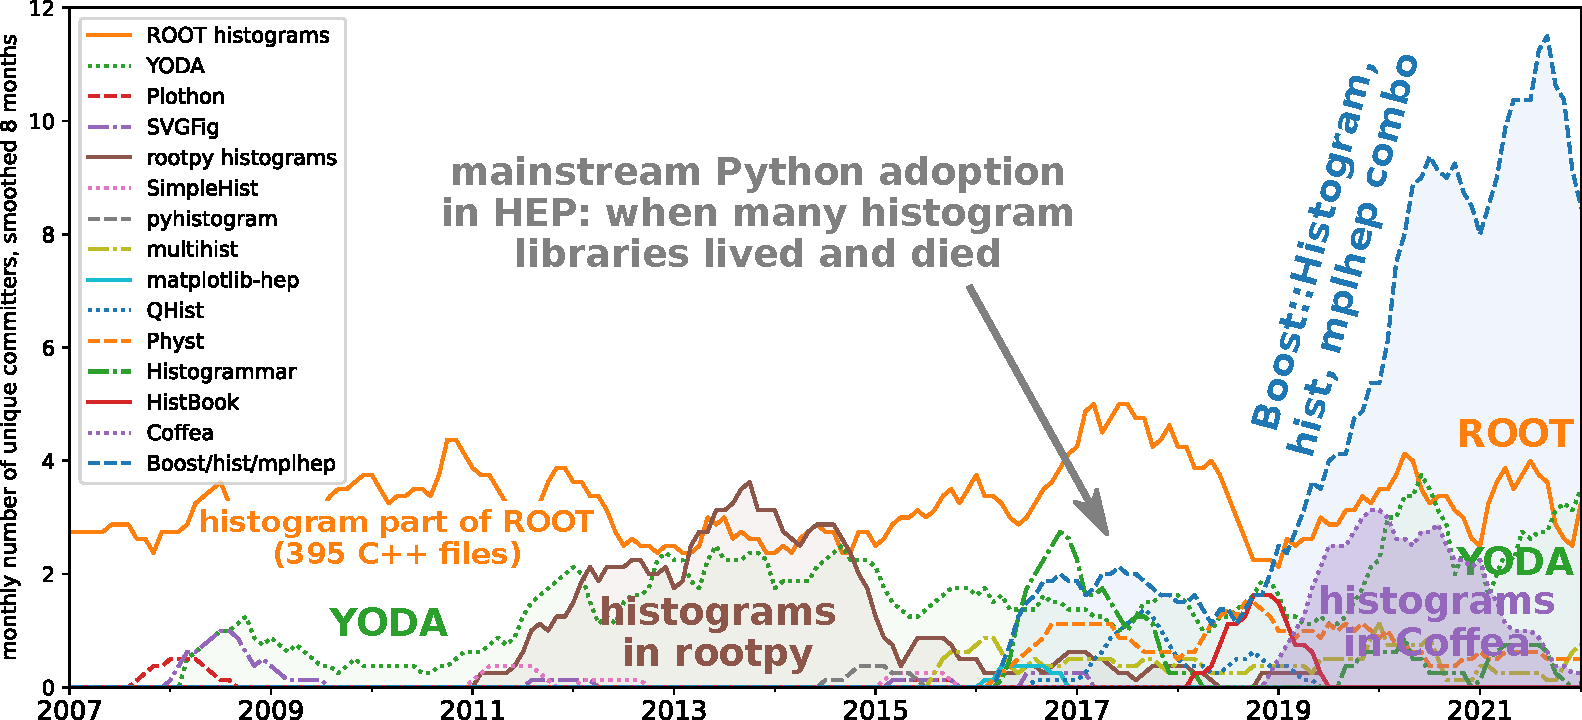
\includegraphics[width=\linewidth]{github-histogram-libraries.pdf}
\end{frame}

\begin{frame}[fragile]{Why combine Boost::Histogram, hist, mplhep?}
\vspace{0.5 cm}
\begin{columns}
\column{0.6\linewidth}
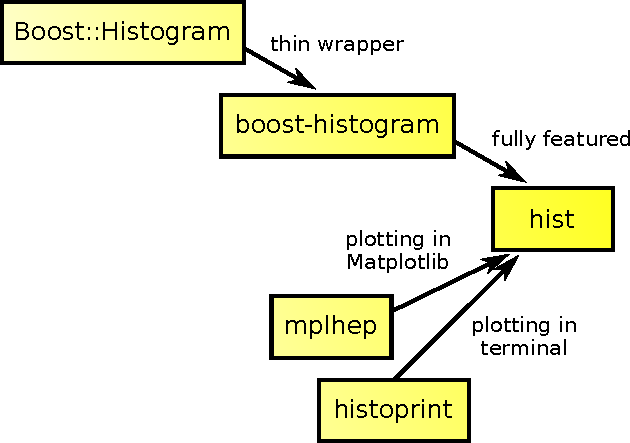
\includegraphics[width=\linewidth]{histogram-convergence.pdf}

\column{0.45\linewidth}
Originally, each of these was developed independently by a single author.

\vspace{0.75 cm}
\begin{uncoverenv}<2->
They each provide a piece of functionality users can get through

\begin{minted}{python}
import hist
\end{minted}
\end{uncoverenv}

\vspace{0.75 cm}
\uncover<3->{Now, 47 developers have contributed to these packages, and 20 contributed to more than one.}
\end{columns}
\end{frame}

\begin{frame}{Consistency maintained through agreed-upon protocols}
\vspace{0.5 cm}
\begin{columns}
\column{1.1\linewidth}
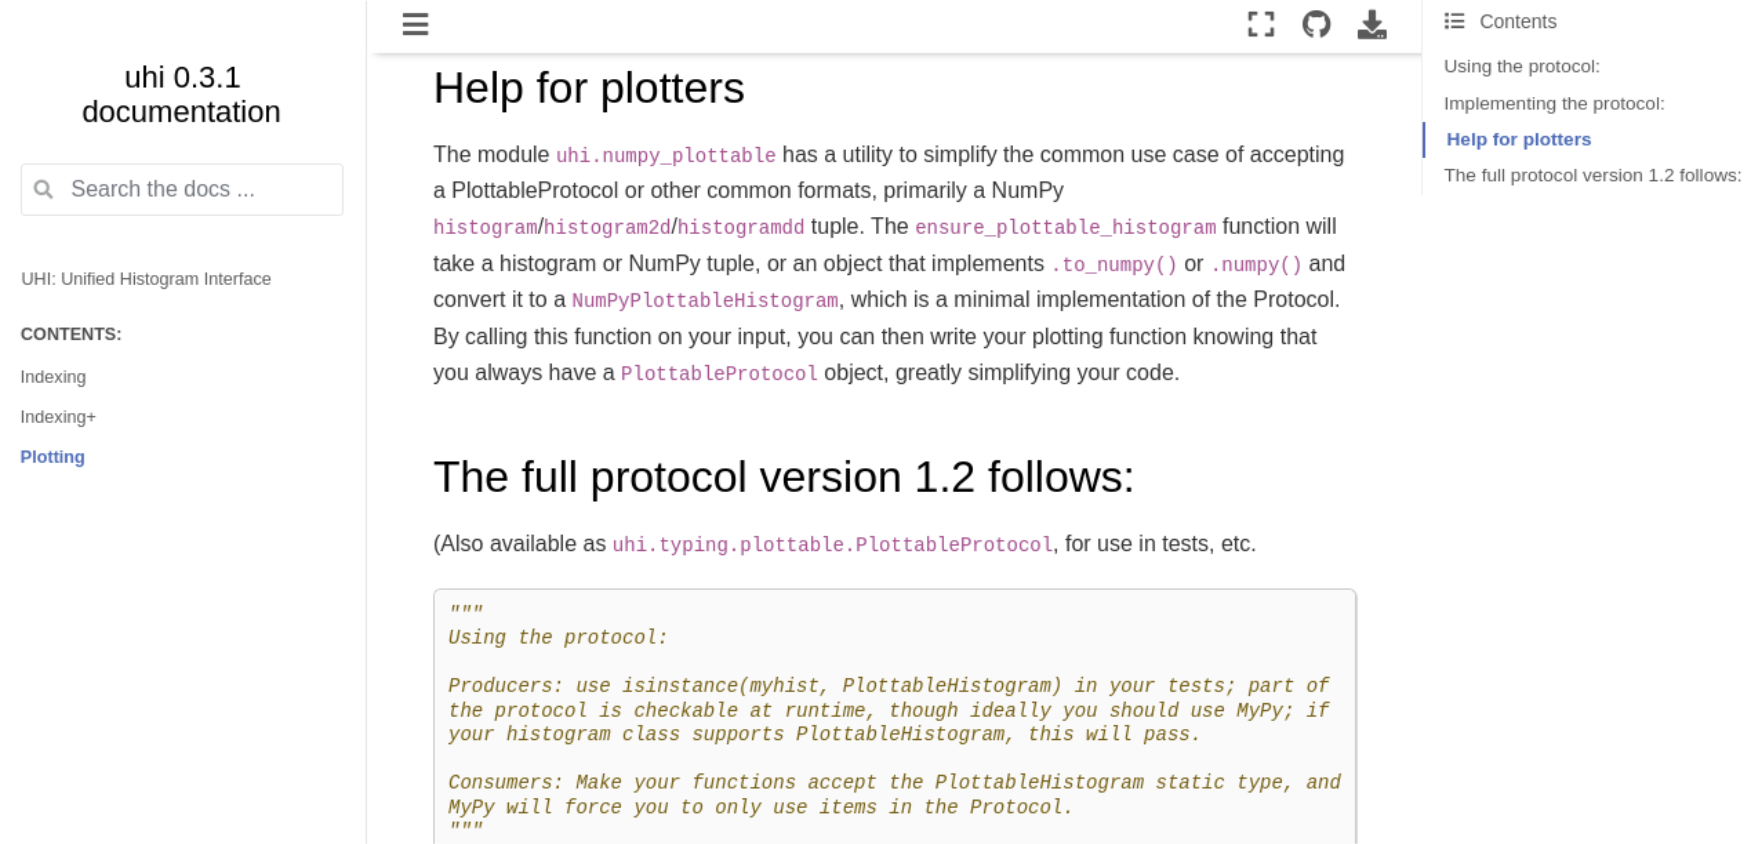
\includegraphics[width=\linewidth]{histogram-protocol-screenshot.png}
\end{columns}
\end{frame}

\begin{frame}{Another need: arrays of non-tabular data}
\large
\vspace{0.25 cm}

Almost all HEP data consists of variable-length lists and nested objects, which would be easiest to describe as JSON (though inefficient). To make use of NumPy-centric tools, we need a way of accessing such data in a NumPy-like way.

\begin{columns}
\column{1.05\linewidth}
\only<1>{
\includegraphics[width=\linewidth]{figures/pivarski-one-slide-summary-0.pdf}}\only<2>{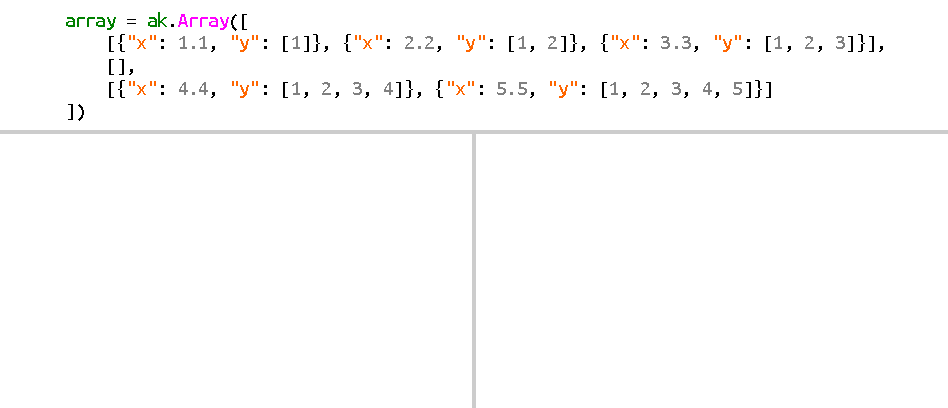
\includegraphics[width=\linewidth]{figures/pivarski-one-slide-summary-1.pdf}}\only<3>{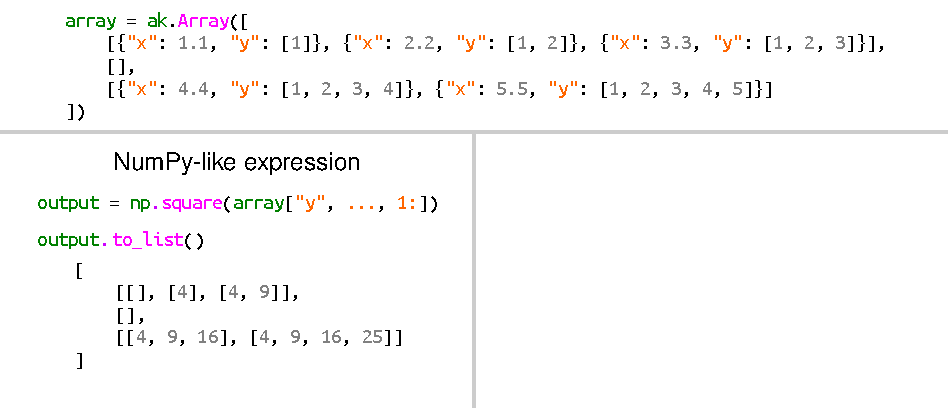
\includegraphics[width=\linewidth]{figures/pivarski-one-slide-summary-2.pdf}}\only<4>{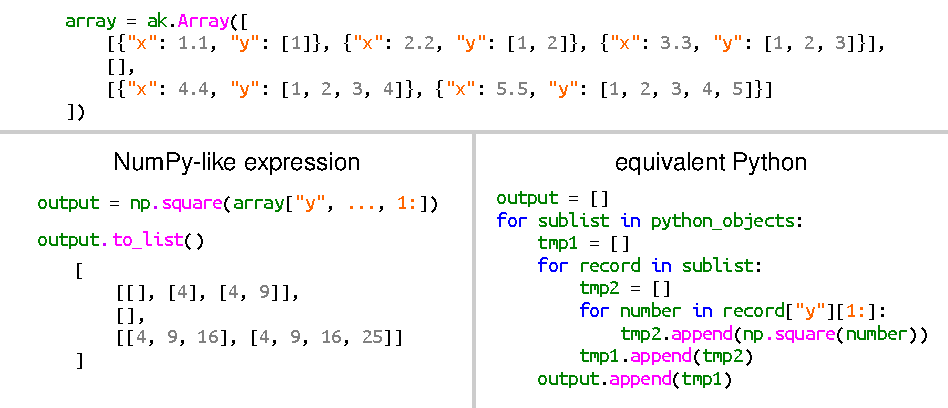
\includegraphics[width=\linewidth]{figures/pivarski-one-slide-summary-3.pdf}}
\end{columns}
\end{frame}

%
\begin{frame}{IRIS-HEP grand challenges test interactions between services and tools}
\vspace{0.35 cm}
\begin{columns}
\column{1.1\linewidth}
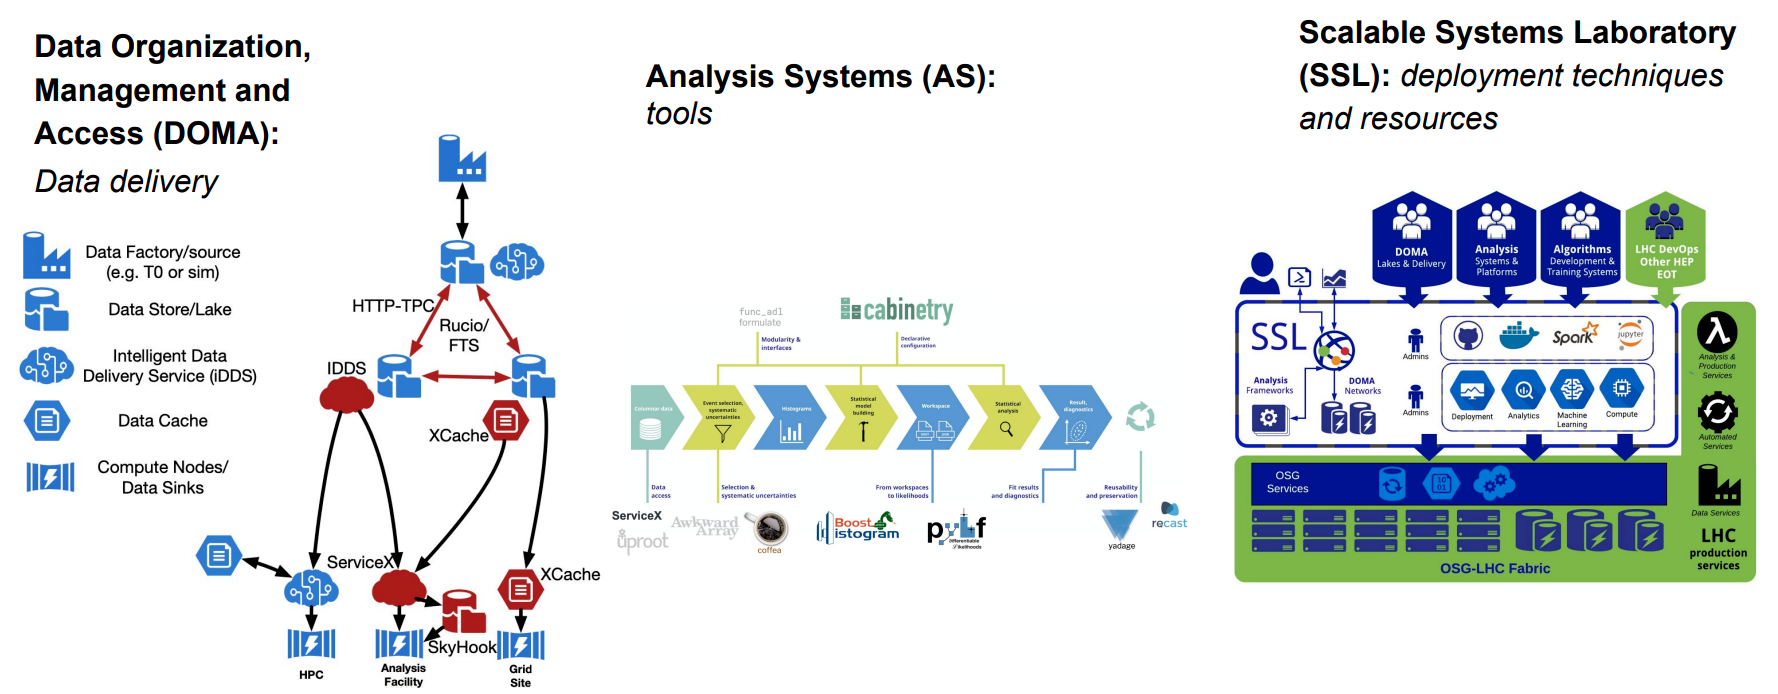
\includegraphics[width=\linewidth]{agc-intersection-of-services-and-tools.png}
\end{columns}
\end{frame}

\begin{frame}{Optimizing Data Delivery}
\begin{center}
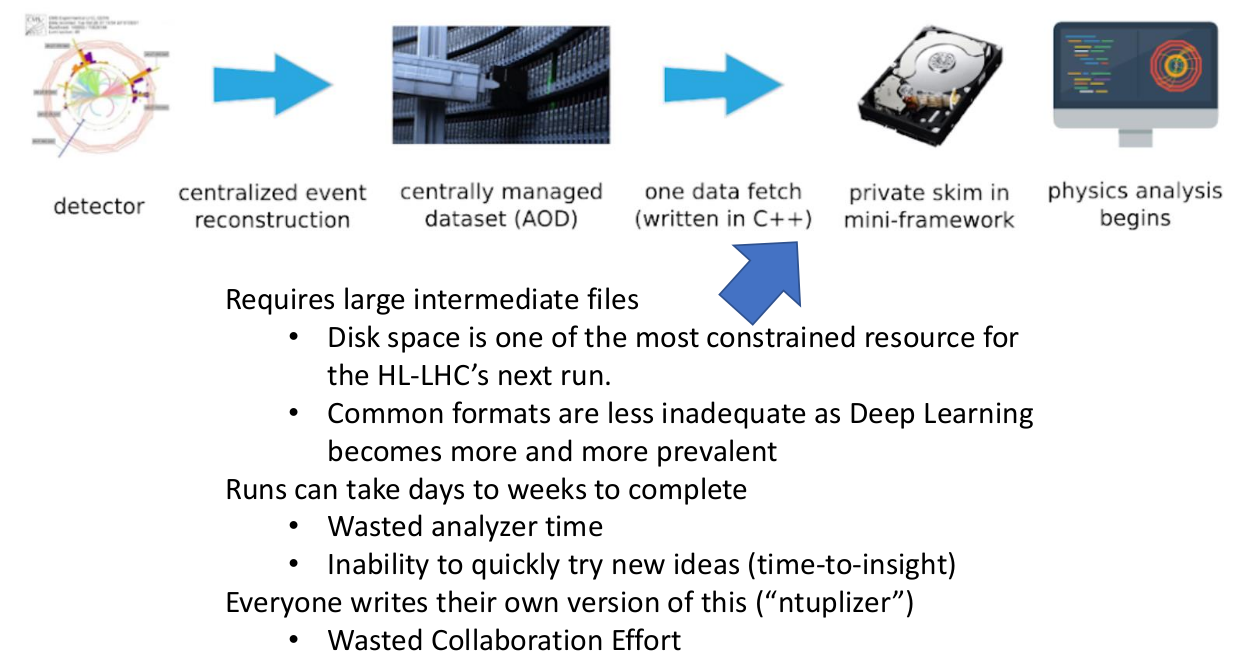
\includegraphics[width=0.95\linewidth]{ServiceX_01.png}
\end{center}
\end{frame}

\begin{frame}{Optimizing Data Delivery}
\begin{center}
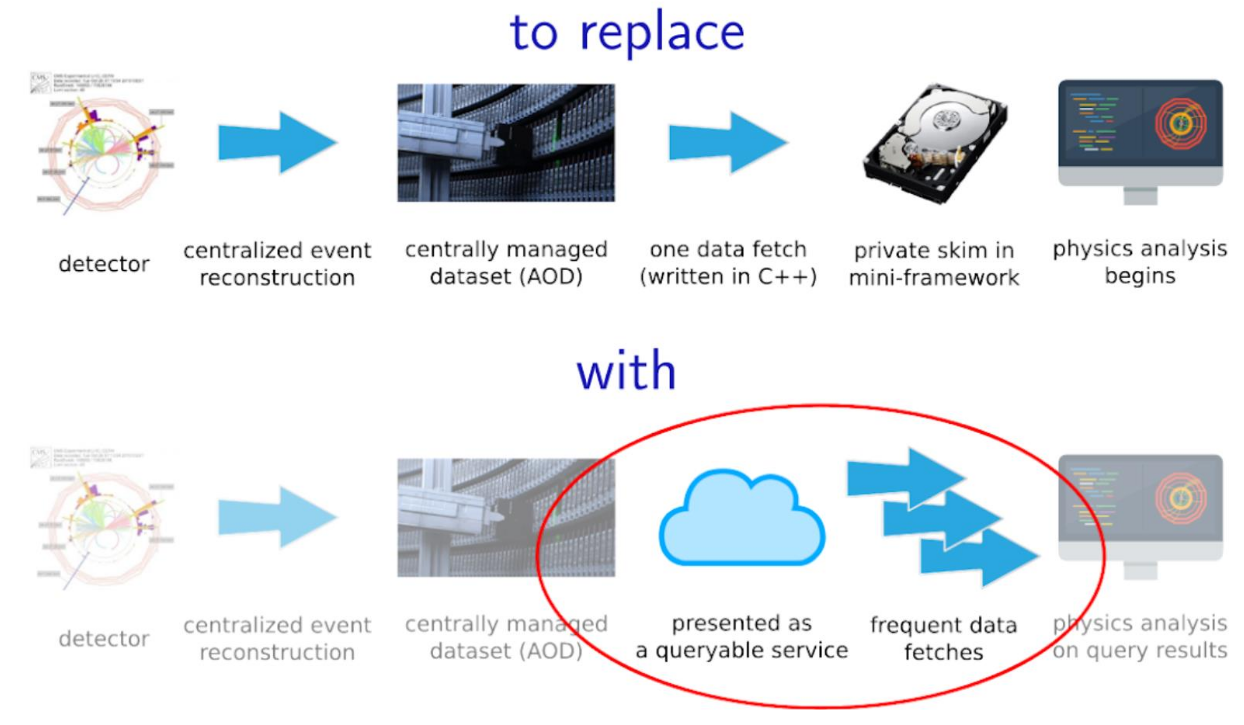
\includegraphics[width=0.95\linewidth]{ServiceX_02.png}
\end{center}
\end{frame}

\begin{frame}{Optimizing Data Delivery}
\vspace{0.1cm}
\begin{center}
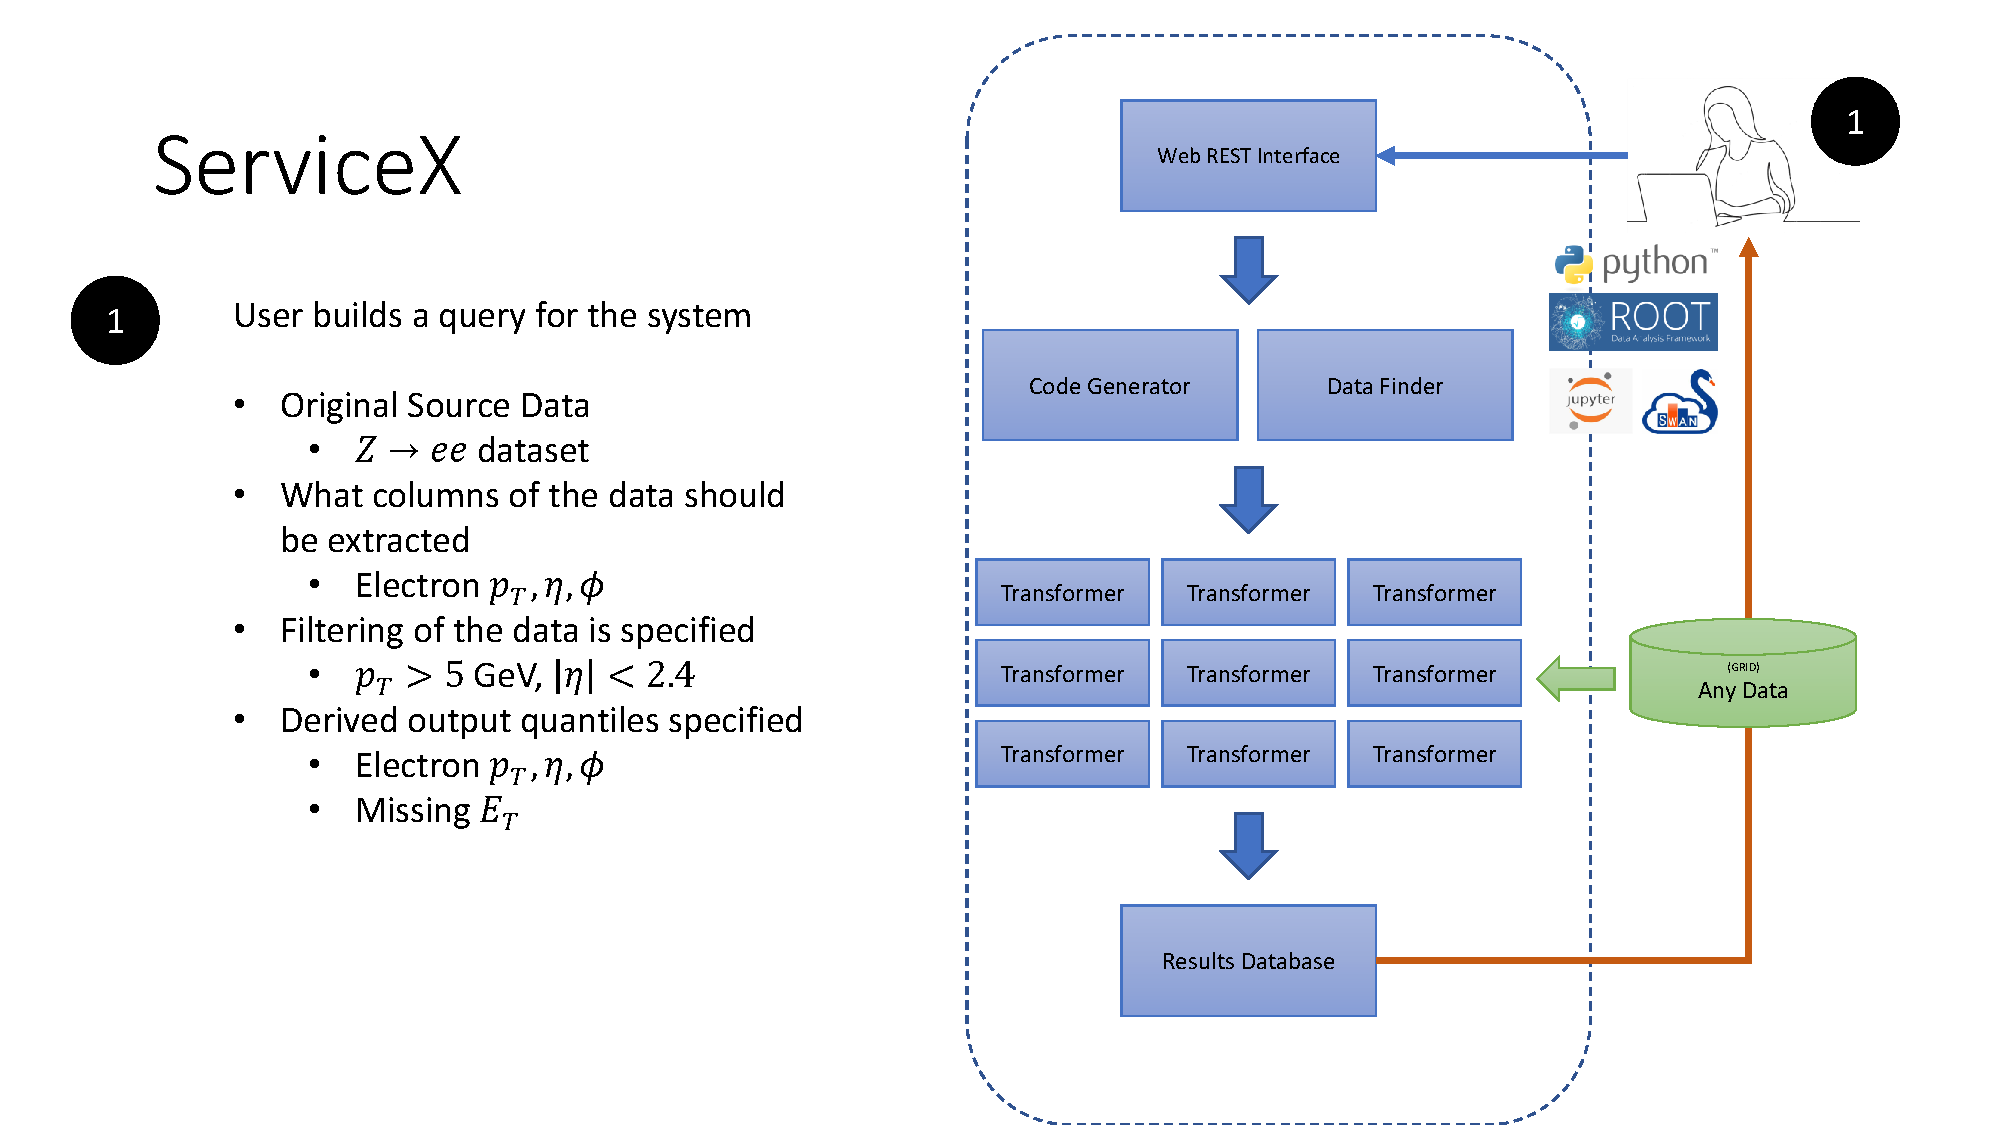
\includegraphics[width=0.95\linewidth]{ServiceX_03.pdf}
\end{center}
\end{frame}

\begin{frame}{Optimizing Data Delivery}
\vspace{0.1cm}
\begin{center}
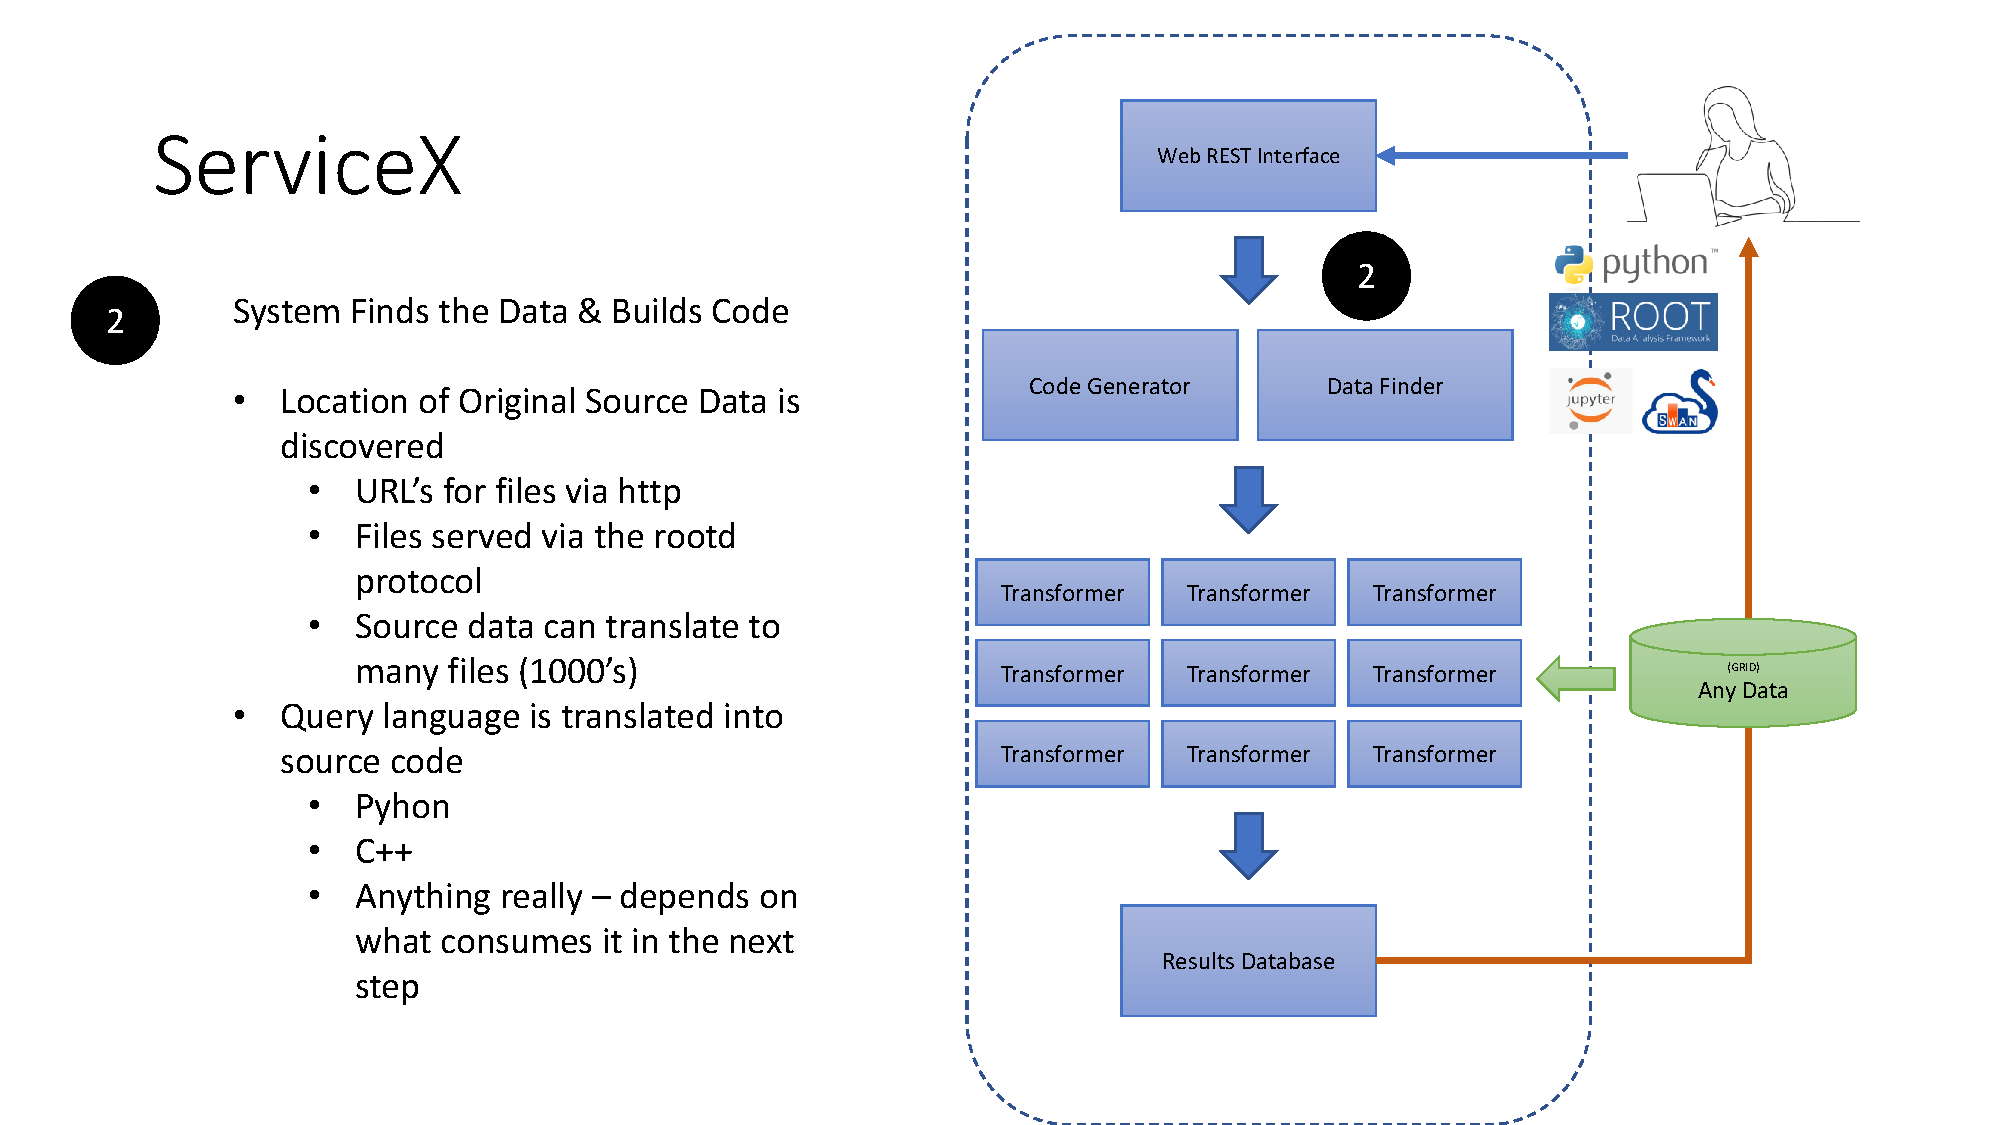
\includegraphics[width=0.95\linewidth]{ServiceX_04.pdf}
\end{center}
\end{frame}

\begin{frame}{Optimizing Data Delivery}
\vspace{0.1cm}
\begin{center}
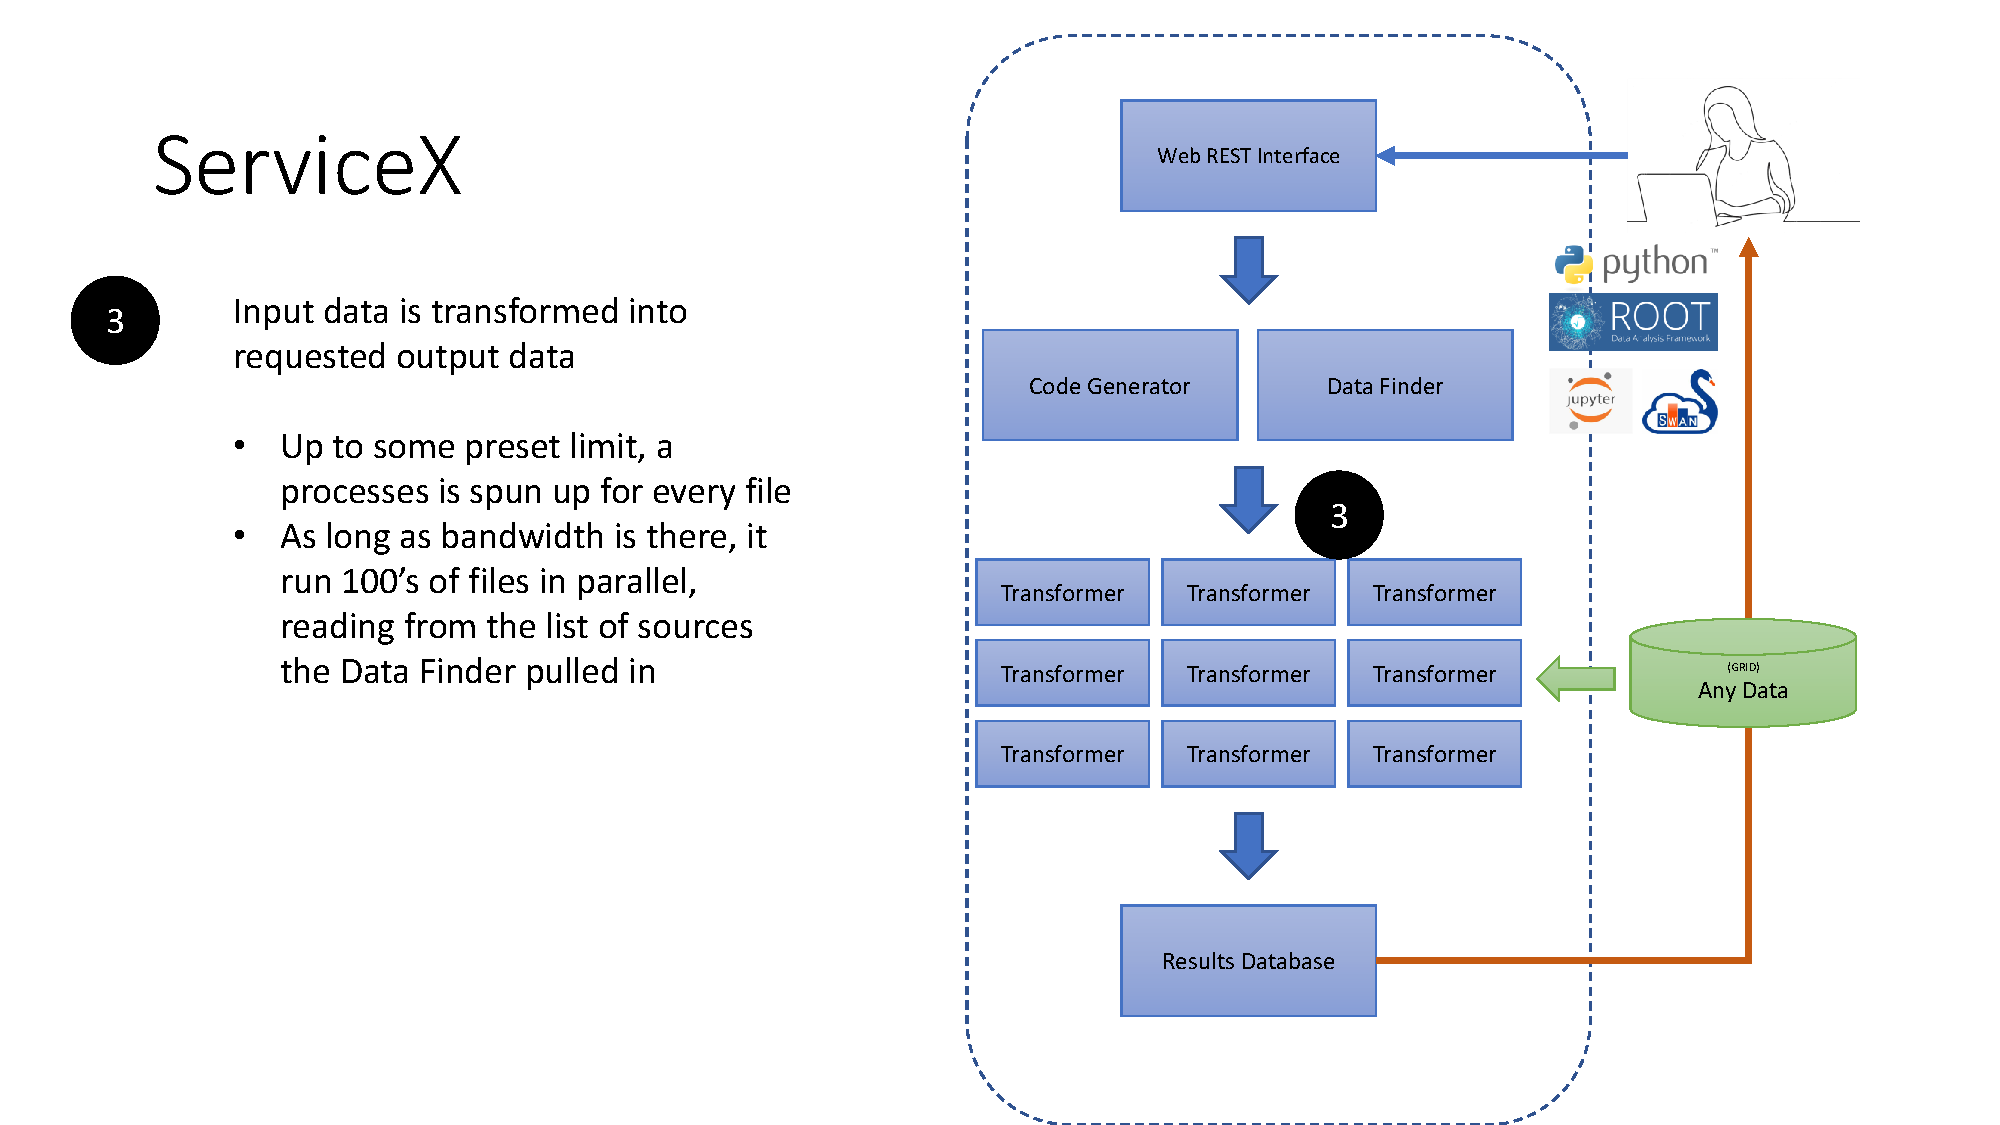
\includegraphics[width=0.95\linewidth]{ServiceX_05.pdf}
\end{center}
\end{frame}

\begin{frame}{Optimizing Data Delivery}
\vspace{0.1cm}
\begin{center}
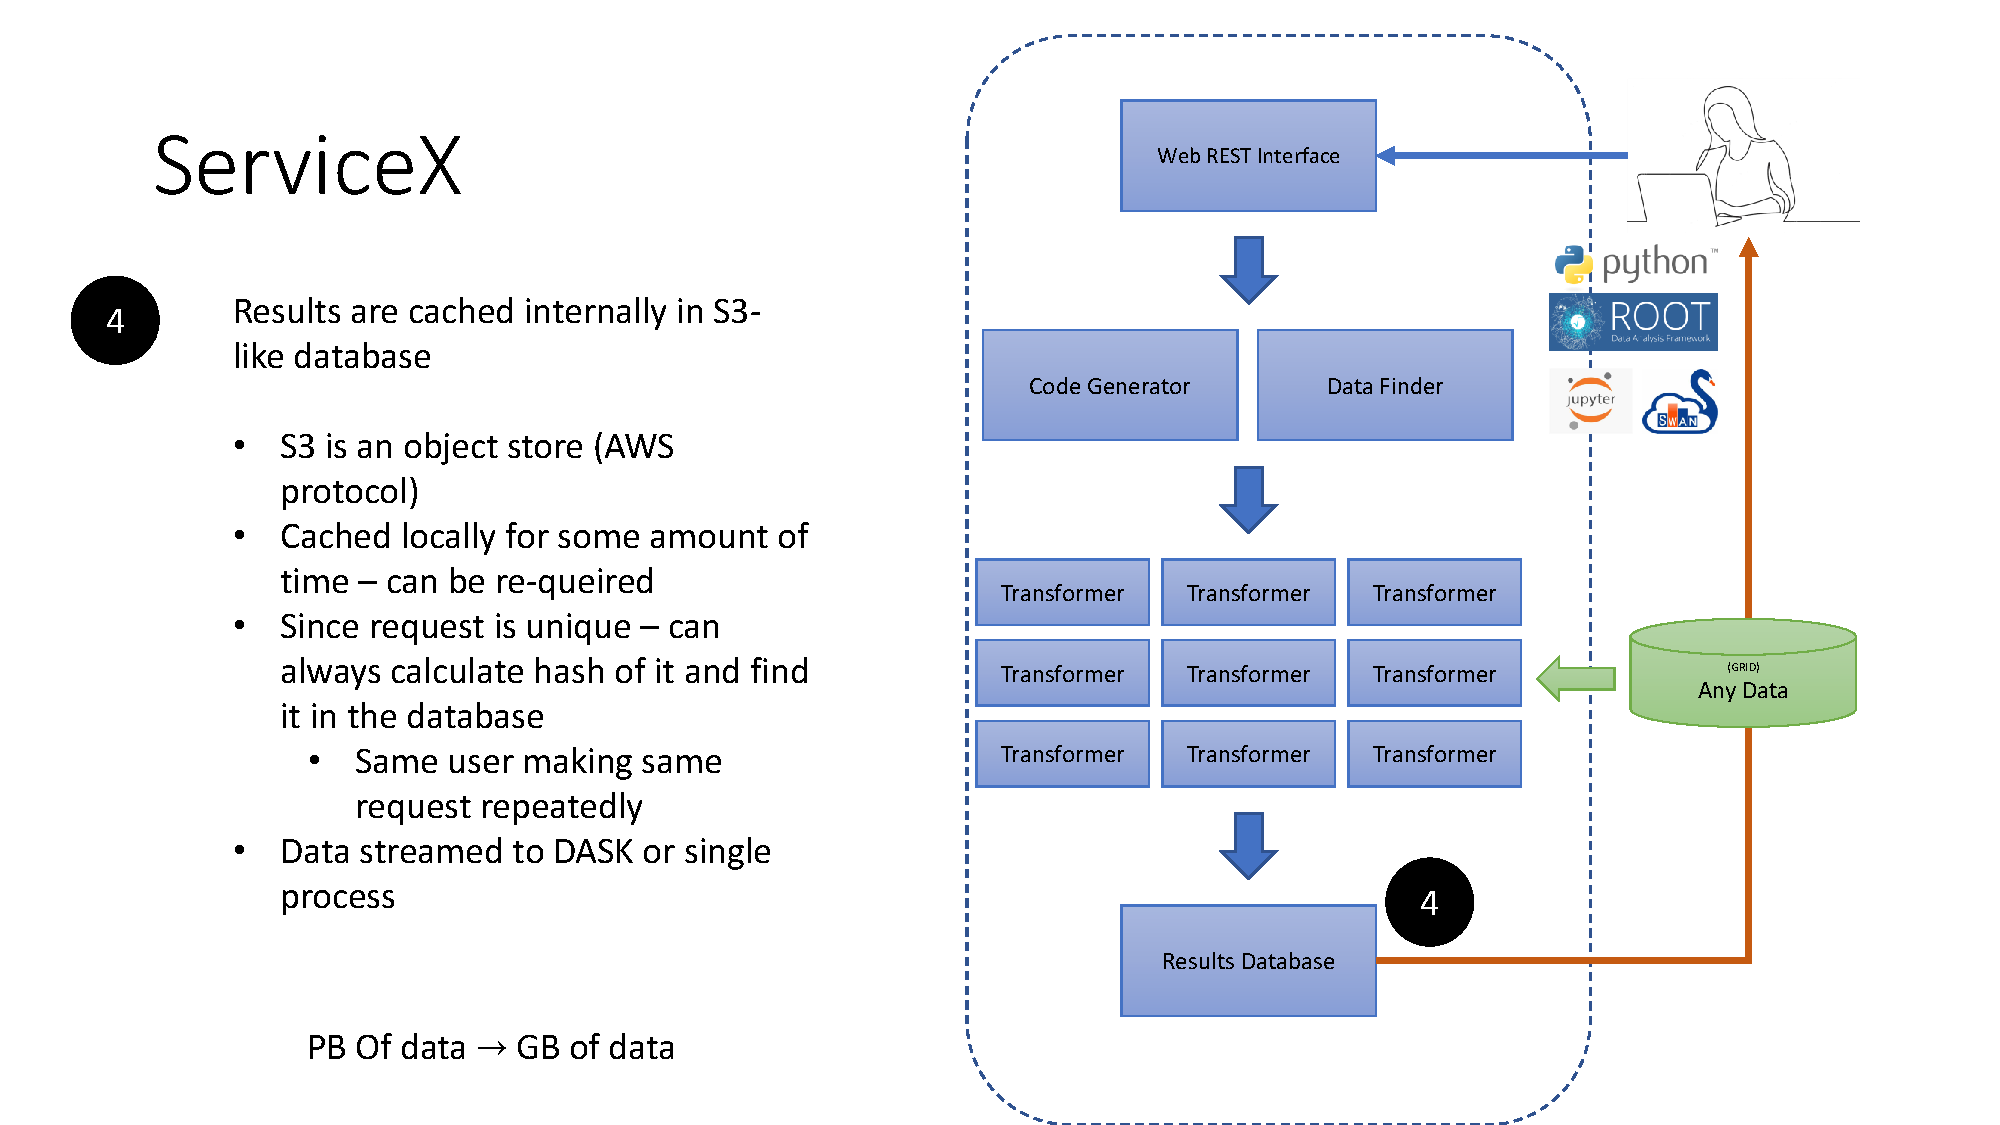
\includegraphics[width=0.95\linewidth]{ServiceX_06.pdf}
\end{center}
\end{frame}

\begin{frame}{Optimizing Data Delivery}
\vspace{0.1cm}
\begin{center}
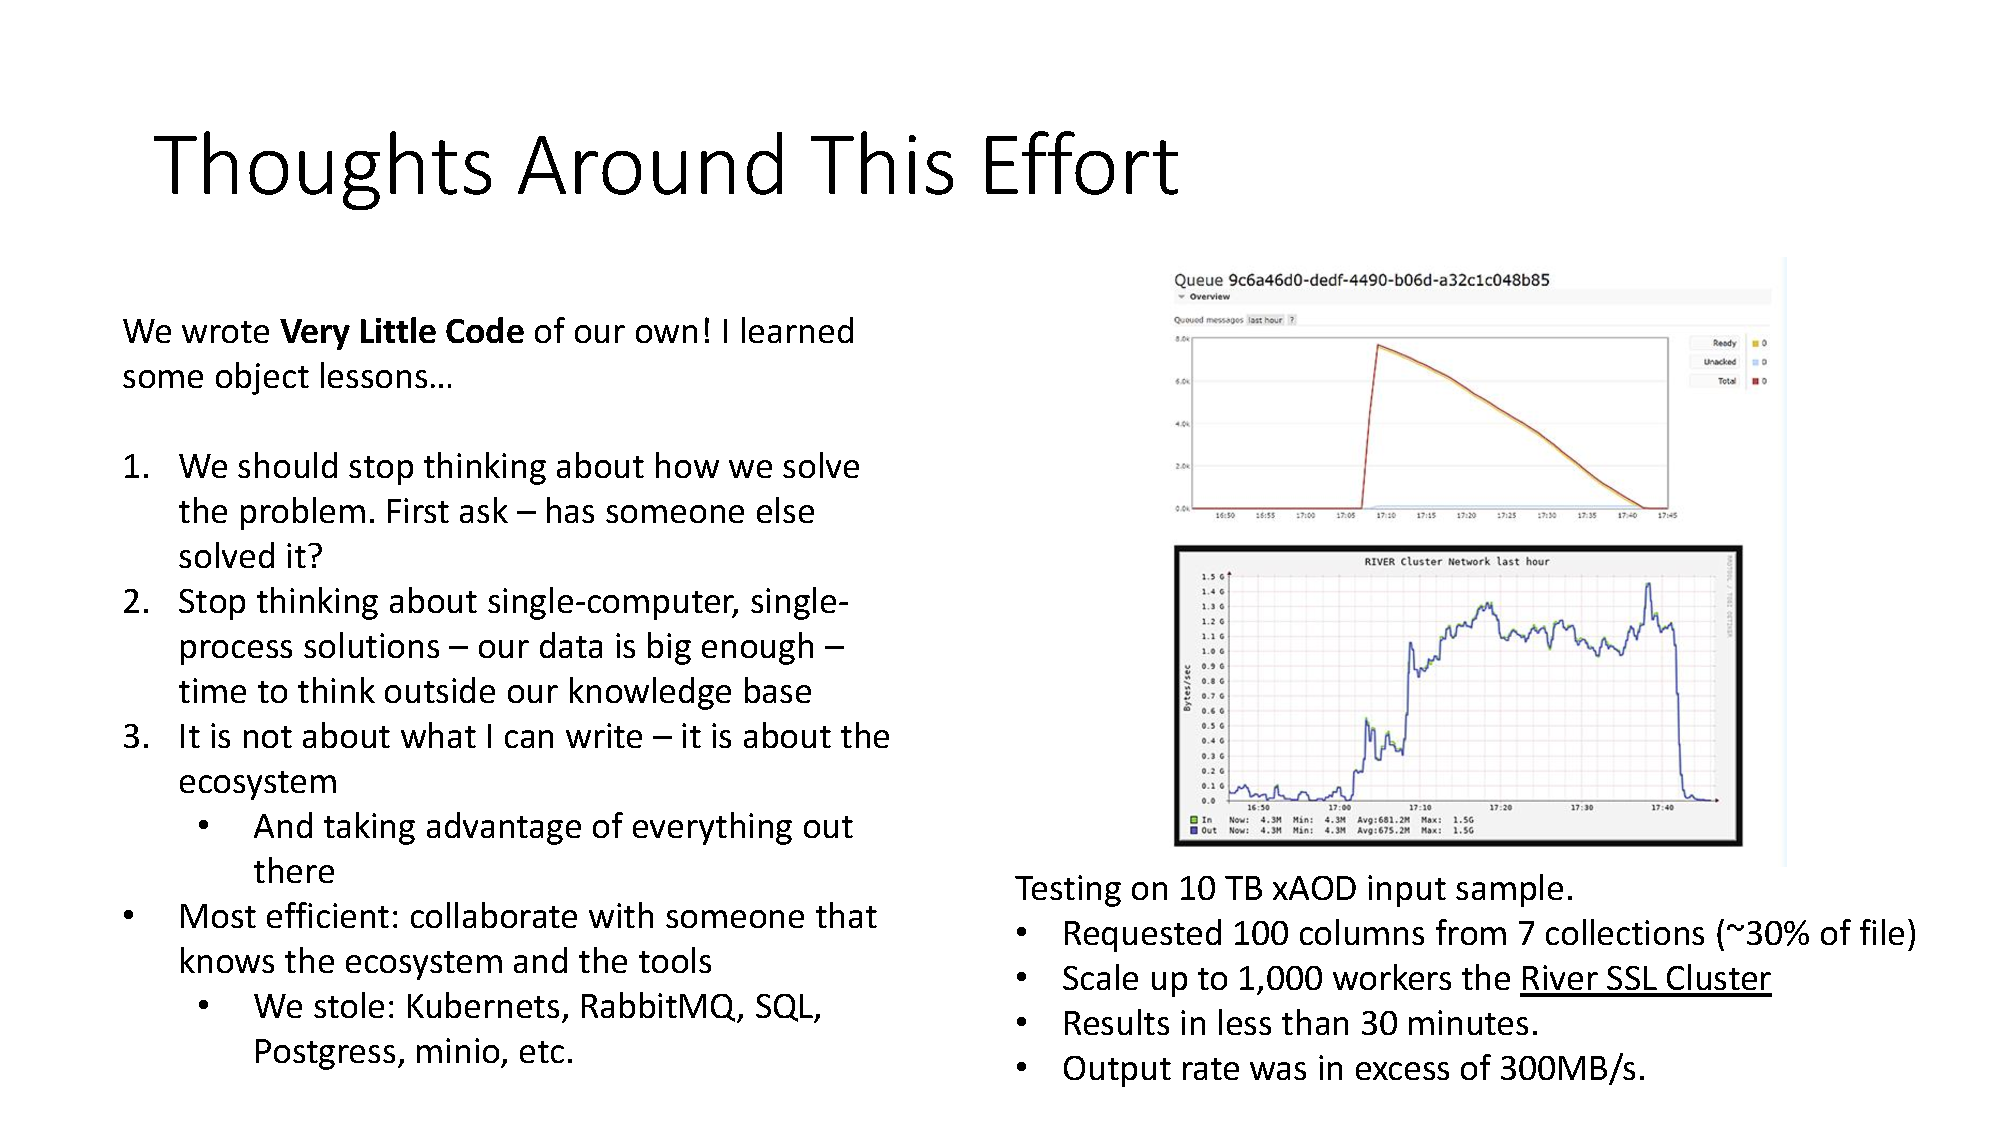
\includegraphics[width=0.95\linewidth]{ServiceX_07.pdf}
\end{center}
\end{frame}


\begin{frame}{Conclusions: Modern Pythonic analysis in HEP is happening now}
\Large
\begin{center}
A confluence of scientific tools and scientists has lead to a feature-complete \textbf{Scikit-HEP} in the last 5 years
\end{center}
\vspace{0.1 cm}

\begin{center}
\href{https://indico.cern.ch/event/613842/contributions/2591057/}{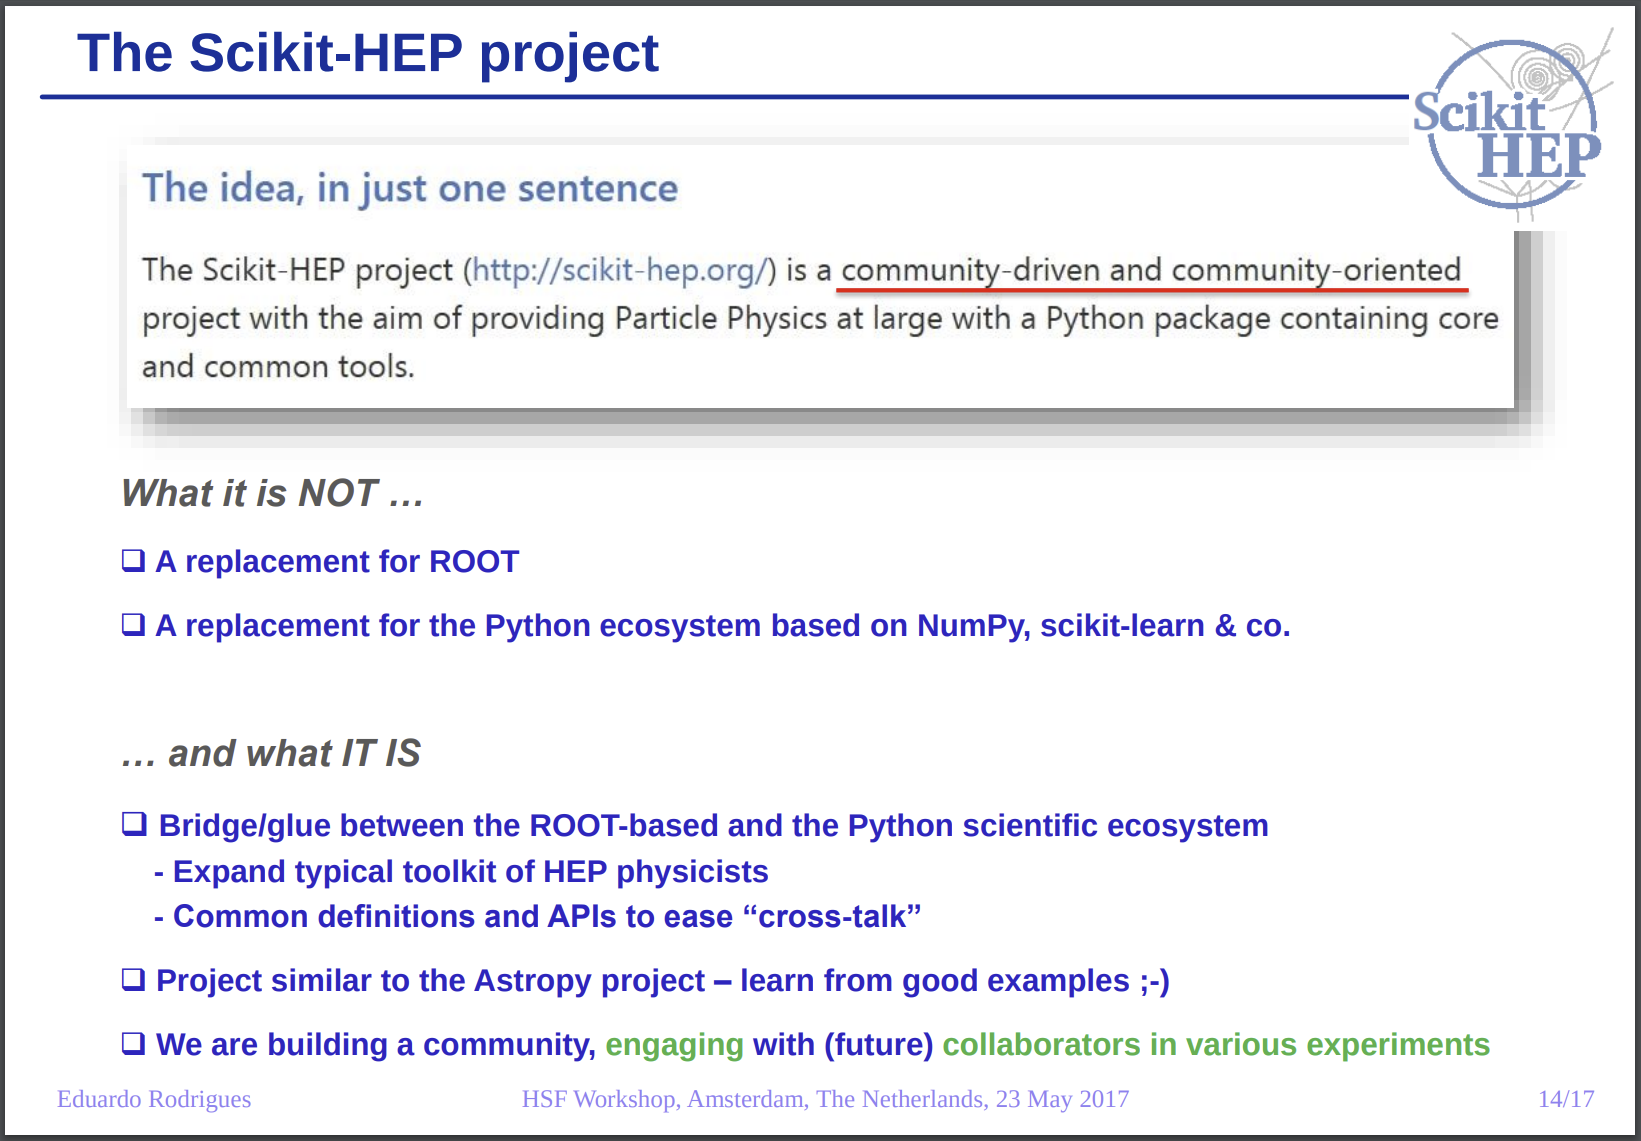
\includegraphics[width=0.625\linewidth]{scikit-hep-in-2017.png}}
\end{center}

\vspace{-1.5 cm}
\hfill \mbox{Eduardo Rodrigues\hspace{-0.5 cm}}
\vspace{1.5 cm}
\end{frame}

\begin{frame}{Conclusions: Modern Pythonic analysis in HEP is happening now}
\Large
\begin{center}
Growing PyHEP \textbf{ecosystem} is enabling analysts in HEP to explore and reduce the time to insight
\end{center}
\vspace{0.1 cm}

\begin{center}
  \href{https://indico.cern.ch/event/1140031/}{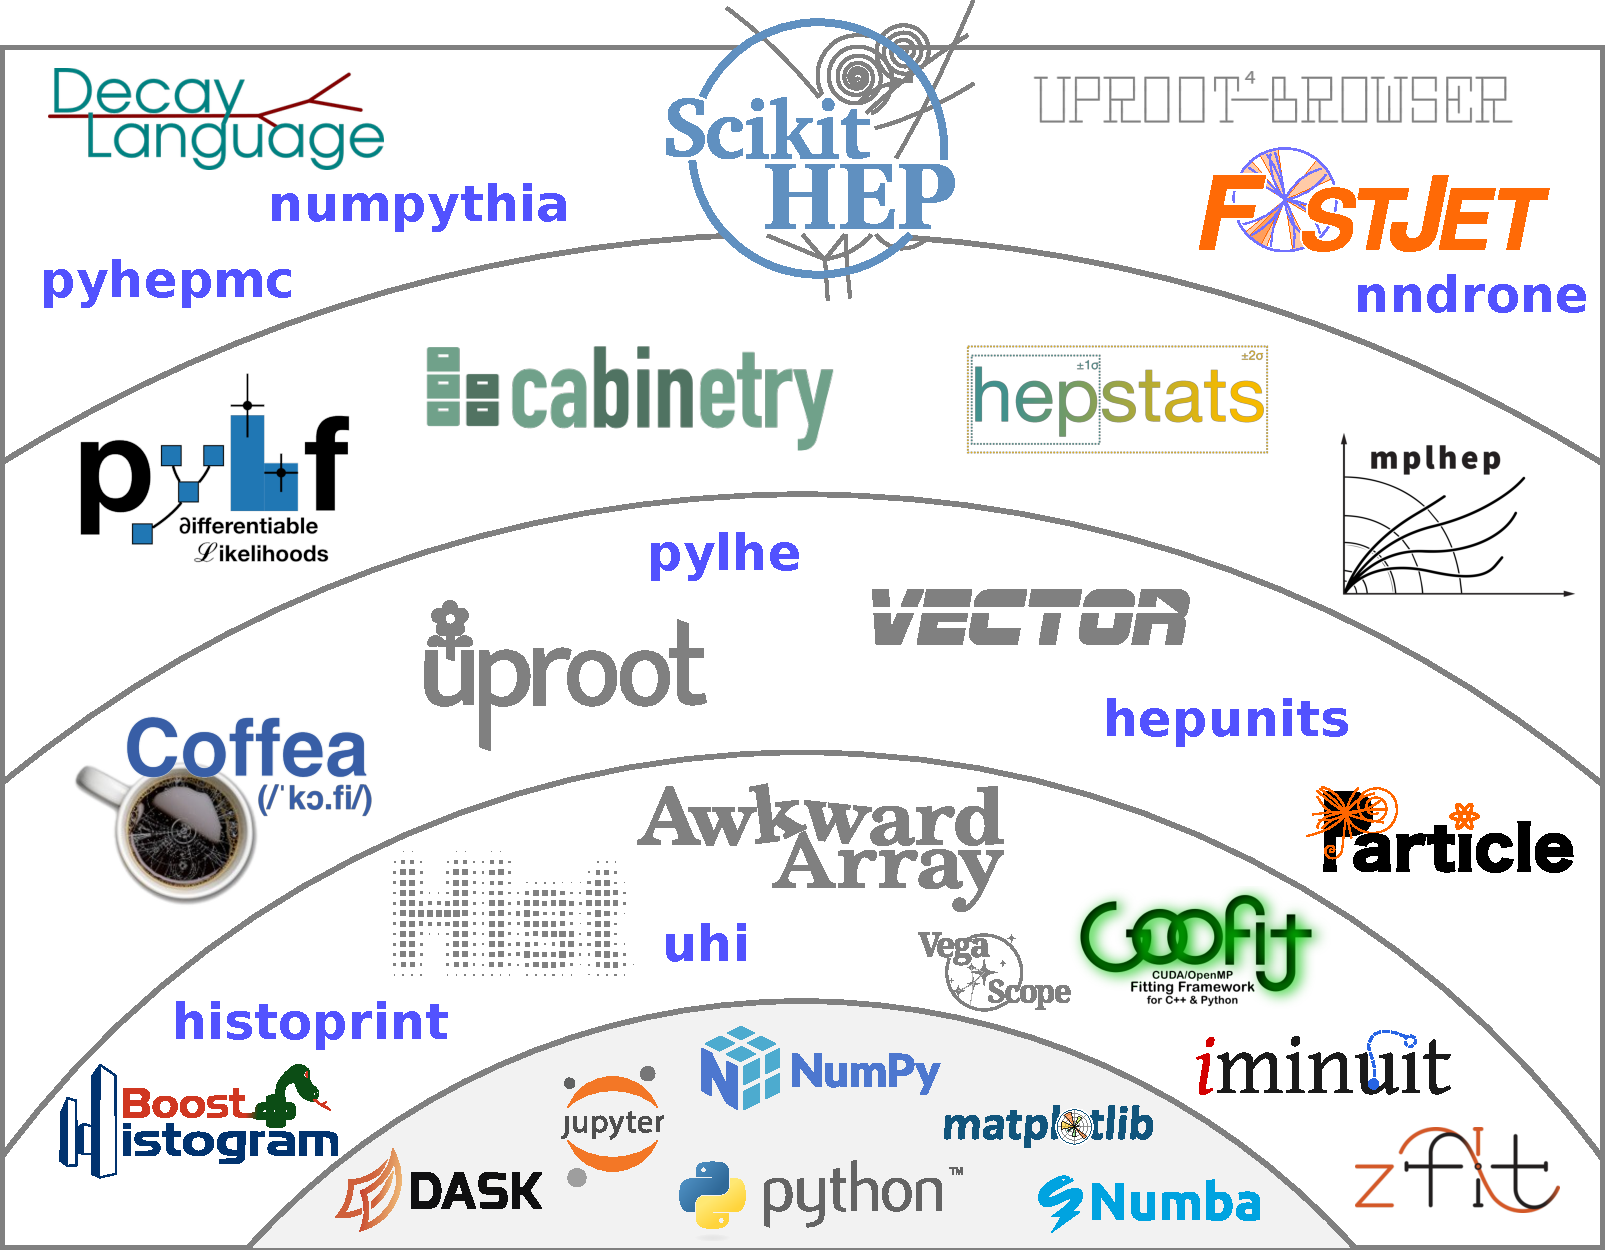
\includegraphics[width=0.55\linewidth]{shells-hep.pdf}}
\end{center}
\end{frame}

\end{document}
